
\section{Evaluation}
\label{sec:evaluation}

We evaluate the Legion type system on three criteria:
\begin{itemize}
\item Expressivity: Can real applications be written (Section~\ref{subsec:expressivity})?
\item Overhead: Does it reduce checking costs (Section~\ref{subsec:overhead})?
\item Scalability: Can it leverage hierarchical scheduling (Section~\ref{subsec:scalability})?
\end{itemize}
%Our evaluation uses a prototype implementation of the Legion language and programming model.
Our prototype implementation has two components: a type checker
for the language introduced in Section~\ref{sec:legioncore} and a C++ runtime library
for executing programs written in the Legion programming model\cite{Legion12}.  All experiments
are conducted on the Keeneland supercomputer\cite{Keeneland}.  Each node of the Keeneland
machine consists of two Xeon 5660 CPUs, three Tesla M2090 GPUs, and 24 GB of DRAM.  Nodes
are connected by a QDR Infiniband interconnect.

\subsection{Expressivity}
\label{subsec:expressivity}
We evaluate Legion on three real-world applications.  To qualitatively gauge the 
expressivity of the Legion type system, we introduce these applications
by describing features of the Legion type system used in their implementations.
The Circuit example was already covered in detail in Section~\ref{sec:example}.

%\subsubsection{Circuit Simulation}
%\label{subsec:circuit}
%Circuit simulates the wires of a large integrated circuit.
% using an RLC model.  
%The computation consists of three phases for each time step: compute the current in each wire using
%an iterative model, updated the charge in each node, and compute the voltage of each node.
%The primary data structure is a large irregular graph, which is
%dynamically partitioned into pieces to enable parallel simulation.
%Our implementation creates separate regions for the wires and
%nodes,  which are recursively partitioned into
%subregions for pieces of the graph.  The node region is partitioned an additional way to 
%describe the sets of ghost nodes required for each piece.  
%The information about each piece of the graph is stored
%in a region relationship that remembers the disjointness information of each piece
%from other pieces.  The tasks for the three phases of the computation use different combinations of
%read, write, and reduce privileges as well as exclusive and simultaneous coherence.

\subsubsection{Fluid Simulation}
\label{subsec:fluid}
Fluid is based on the {\tt fluidanimate} benchmark from the PARSEC 
suite\cite{bienia11benchmarking}.  Fluid simulates the flow of an incompressible fluid
using particles that move within a regular grid of cells.  To perform operations in 
parallel the array of cells is partitioned.  Unlike
Circuit, Fluid creates and partitions regions before
allocating cells in them (i.e., partition-then-allocate).  Another difference is that Fluid
maintains separate regions for ghost cells rather using multiple partitions of
the regions containing shared data.  Region relationships are used for remembering
which regions are required for each grid.

\subsubsection{Adaptive Mesh Refinement}
\label{subsec:amr}
The third application is a Legion port of an adaptive mesh refinement (AMR) benchmark 
from BoxLib \cite{BoxLib}.  The algorithm solves the two
dimensional heat diffusion equation on a grid of cells using three levels of refinement with sub-refinements
randomly placed on the surface.  
%For each time step in the application, cells at the boundary of
%a refinement are interpolated from cells at a coarser level of refinement, energy fluxes between
%cells are computed, energy is transferred, and cells at a coarser level of refinement are restricted
%to the values of refined cells.  
Every level of refinement uses a separate region, which is partitioned several ways to support multiple views of
the cells.  One partitioning separates cells into pieces that can be updated in
parallel.  Additional partitions are created for viewing data from coarser and finer levels of
the simulation.  Two types of region relationships are created: one for describing the pieces at 
each level of refinement, and another for describing the relationship between pieces at different
levels of refinement.  
%These region relationships capture both intra- and inter-level disjointness information.  
The dynamic nature of AMR requires that regions be created and partitioned at runtime.  
%The many ways in which cells are used also requires multiple simultaneous
%partitions of regions.

These applications show Legion is capable of 
expressing applications with both regular (Fluid, AMR) and irregular (Circuit) pointer data structures.
Being able to dynamically create and partition regions at runtime is crucial to Legion's
ability to handle applications that make runtime decisions about data organization (AMR).  Legion
is able to capture both allocate-then-partition (Circuit) and partition-then-allocate (Fluid) algorithms. 
Having multiple partitions of regions is necessary for describing the many ways 
that data can be accessed (Circuit, AMR).  All the types of privileges and coherence we have
described are needed in different applications.  Region relationships
are used in all applications. %, region relationships convey disjointness information.
% despite
%regions being a first-class feature that cannot be fully tracked statically.

\subsection{Checking Overhead}
\label{subsec:overhead}
Our first Legion implementation consisted of a C++ library of Legion primitives
\cite{Legion12} with no checking of region memory accesses.  
When testing applications we frequently encountered memory corruption due to
illegal region accesses caused by application bugs.
In many cases, this corruption occurred between nodes in the cluster or on 
GPUs, environments for which debugging tools are primitive at best.
%  Finding these bugs required either multiple {\tt gdb} sessions 
%for observing execution on different nodes simultaneously or using {\tt printf} for debugging on
%GPUs.  
To locate the application bugs causing these illegal accesses, we initially added 
dynamic checks on  all region accesses for both CPUs and GPUs.  
Unsurprisingly, these checks added considerable runtime overhead.  
To preserve the benefit of checking every access, but eliminate the cost of dynamic checks we implemented the type, privilege, and coherence checker we have described. 
We then rewrote all of our applications in this language and used our type checker to verify them.  Once the applications type checked we were
able to safely elide all the dynamic region access checks.

%\begin{figure}
%\subfigure[48 Piece Data Set]
%{
%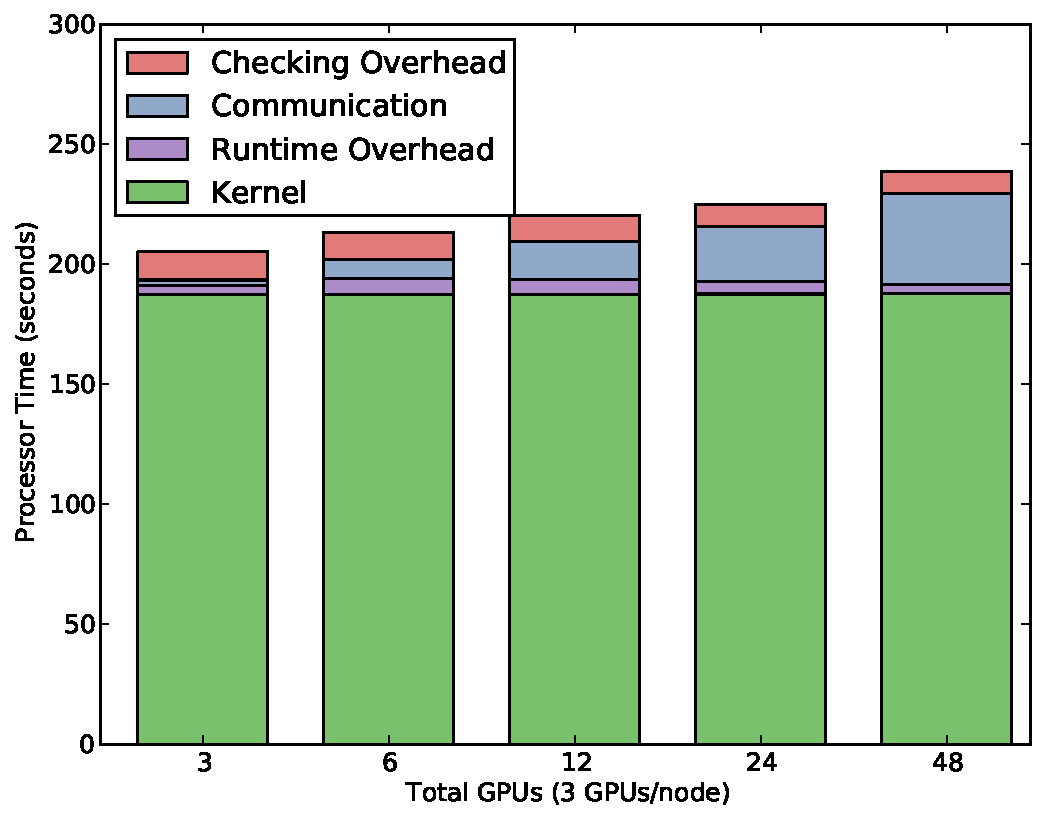
\includegraphics[scale=0.4]{figs/circuit_48_popl.pdf}
%\label{fig:ckt48}
%}
%\subfigure[96 Piece Data Set]
%{
%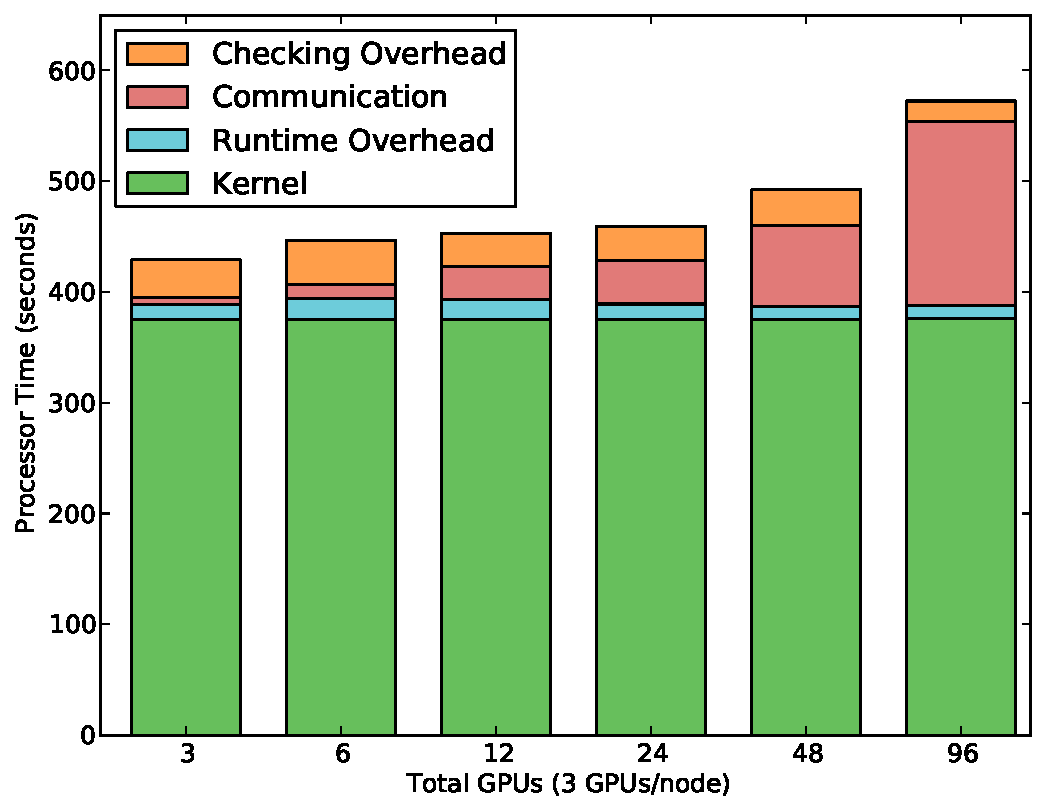
\includegraphics[scale=0.4]{figs/circuit_96_popl.pdf}
%\label{fig:ckt96}
%}
%\caption{Checking overhead of the Circuit simulation.\label{fig:ckt_overhead}}
%\end{figure}

\begin{figure}
\begin{center}
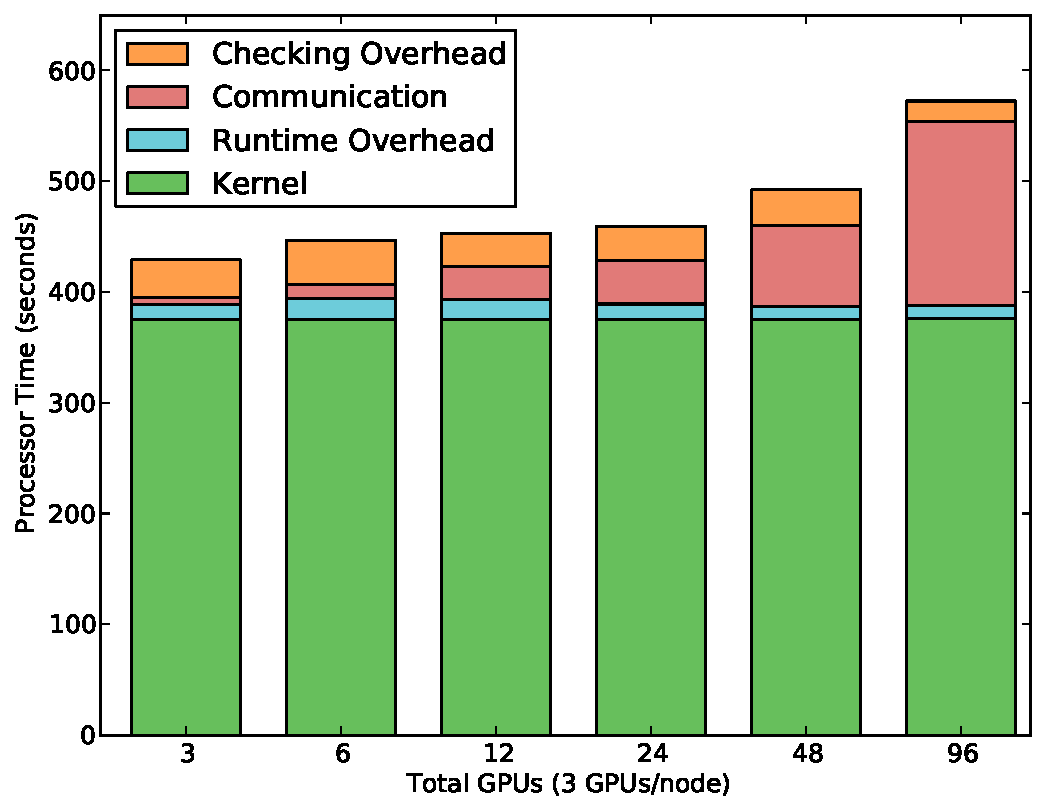
\includegraphics[scale=0.33]{figs/circuit_96_popl.pdf}
\end{center}
\vspace{-2mm}
\caption{Overhead for the Circuit simulation with 96 total pieces.\label{fig:ckt_overhead}}
\vspace{-6mm}
\end{figure}

\begin{figure}
\begin{center}
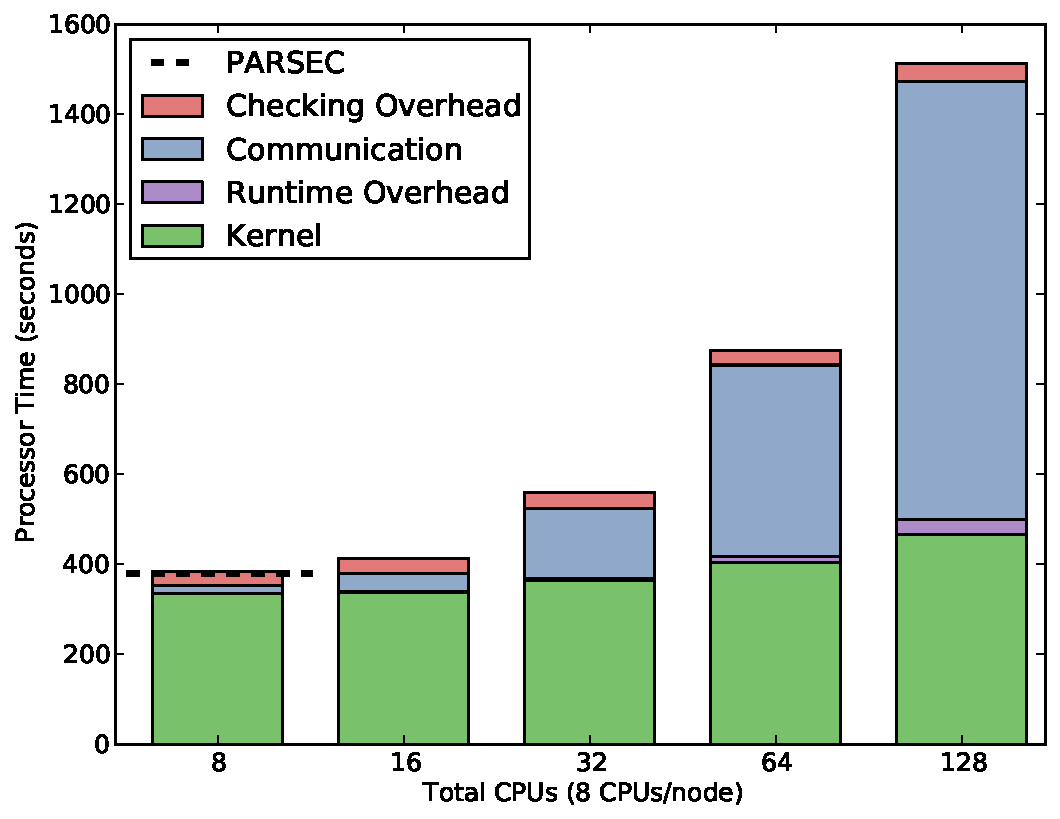
\includegraphics[scale=0.33]{figs/fluid_19200_popl.pdf}
\end{center}
\vspace{-2mm}
\caption{Overhead for the Fluid simulation with 19200 cells.\label{fig:fluid_overhead}}
\vspace{-6mm}
\end{figure}

Figures~\ref{fig:ckt_overhead}, \ref{fig:fluid_overhead}, and \ref{fig:amr_overhead} show 
the total time spent by all CPUs and GPUs in each phase of the application.  The topmost
component of each bar shows the overhead added by the dynamic checks.  In 
each figure the problem size stays the same as the number of processors increases
(strong scaling).  Figure~\ref{fig:amr_overhead} includes multiple problem sizes to show
how overhead is affected by changing problem size (weak scaling).  For cases where there
is an existing implementation to compare against we have included a dotted line indicating
baseline performance.  In a few cases (Figures~\ref{fig:fluid_overhead} and 
\ref{fig:amr4096}) checking overhead is the difference
between better and worse performance than the baseline.  For an explanation of overall
performance relative to the baseline implementations see \cite{Legion12}.

\begin{figure}
\begin{center}
\subfigure[4096 cells per dimension]
{
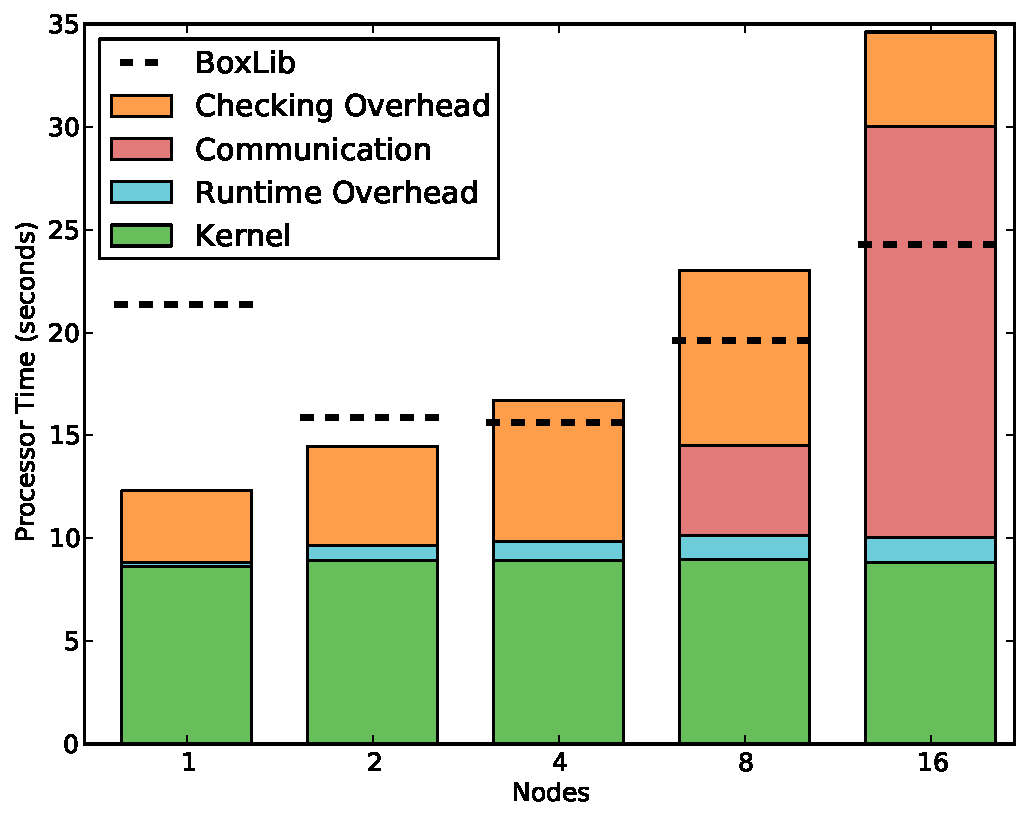
\includegraphics[scale=0.33]{figs/amr_4096_popl.pdf}
\label{fig:amr4096}
}
\subfigure[8192 cells per dimension]
{
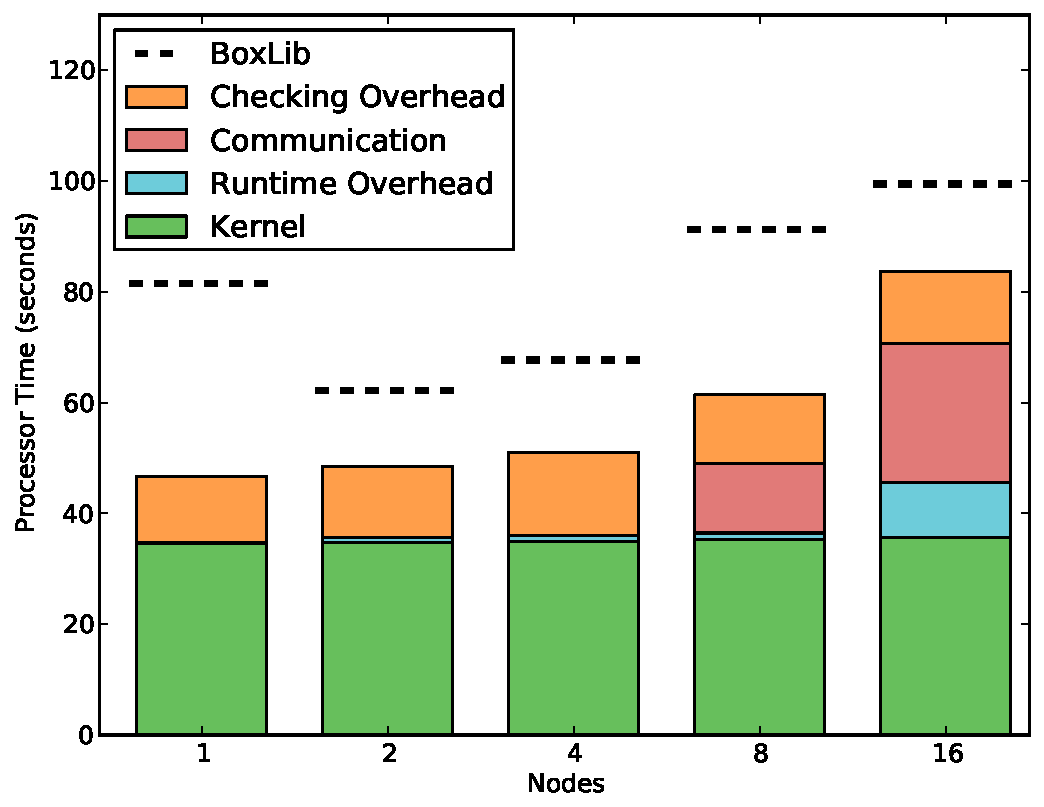
\includegraphics[scale=0.33]{figs/amr_8192_popl.pdf}
\label{fig:amr8192}
}
\subfigure[16384 cells per dimension]
{
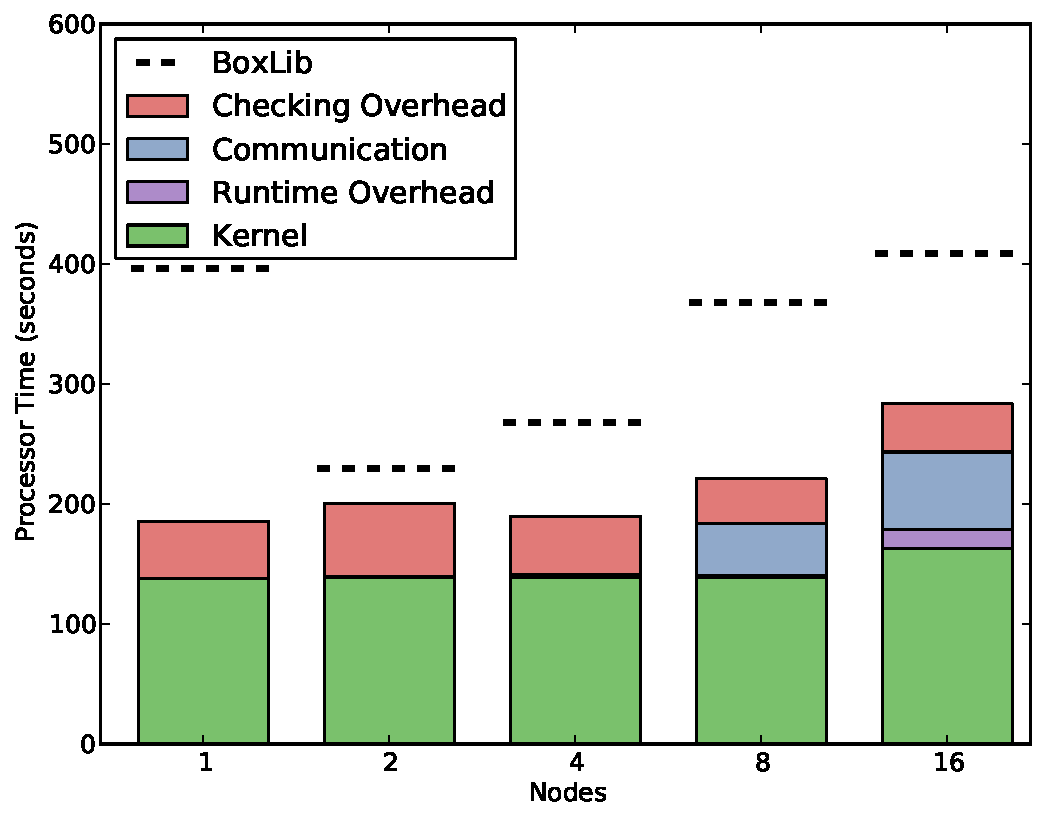
\includegraphics[scale=0.33]{figs/amr_16384_popl.pdf}
\label{fig:amr16384}
}
\end{center}
\vspace{-2mm}
\caption{Overhead for the AMR application.\label{fig:amr_overhead}}
\vspace{-6mm}
\end{figure}

In addition to total processor overhead, we also measured performance gain from eliding checks in 
terms of wall-clock time.  Since most region accesses occur in leaf tasks the checks parallelize 
well.  Wall-clock performance gains from eliding memory checks ranged from 1-10\%, 1-15\%, 
and 2-71\% for Circuit, Fluid, and AMR respectively.  Performance gains for AMR were larger than
the other applications because AMR was already memory bound and the additional checks intensified
memory pressure.  For the GPU kernels in the Circuit application checking required up to 8 additional 
registers per thread.  While the GPU kernels in Circuit were not bound by 
available on-chip memory, kernels that are would be susceptible to extreme performance 
degradation due to the extra registers required for checking.  We also measured the overhead
of the dynamic checks associated with checking task call privileges but found them to be negligible,
demonstrating that runtime non-interference checks are inexpensive in Legion.
% relative to the overhead of region access checks.

\subsection{Scalability}
\label{subsec:scalability}
The scalability of Legion derives directly from Theorem~\ref{thm:hiersched}.  This 
theorem proves it is safe for the runtime to only perform dependence checks between two
tasks that share the same immediate parent task instead of having to consider all
possible interactions with other tasks anywhere in the system.  Since all tasks that
share the same immediate parent are all created on the node where the parent is executing,
all dependence checks and scheduling decisions can be performed locally with no inter-processor communication.  
Without this property the runtime would be forced to inform all other processors in the system 
of every task that it launches using expensive broadcasts. 

Figures~\ref{fig:ckt_overhead}, \ref{fig:fluid_overhead}, and \ref{fig:amr_overhead} show that
the overhead of the Legion runtime is always less than 7\% of the total execution time
of the applications.  In some applications communication doesn't scale well, but this is
a result of the algorithm chosen by the programmer, not the Legion runtime.
Even in the case of the Circuit application, which exhibits quadratic communication scaling, the Legion
runtime is able to achieve a 62.5X speedup on 96 GPUs over a hand-coded single GPU implementation\cite{Legion12}.

